
\documentclass{article}
\usepackage[spanish]{babel}
\usepackage{graphicx}
\usepackage{listings}
\setlength{\parindent}{0pt}
\setlength{\parskip}{3mm}
\usepackage[numbers]{natbib}
\usepackage{color}
\usepackage{booktabs}
\usepackage{subfigure}
\usepackage{pdfpages}


\begin{document}

\includepdf[pages=1-1]{pdfrevisados/MiTesis.pdf}

\section{Introdución}

En el portafolio aparece la retroalimentación de la profesora a las tareas de clase, con las correcciones realizadas a las mismas.


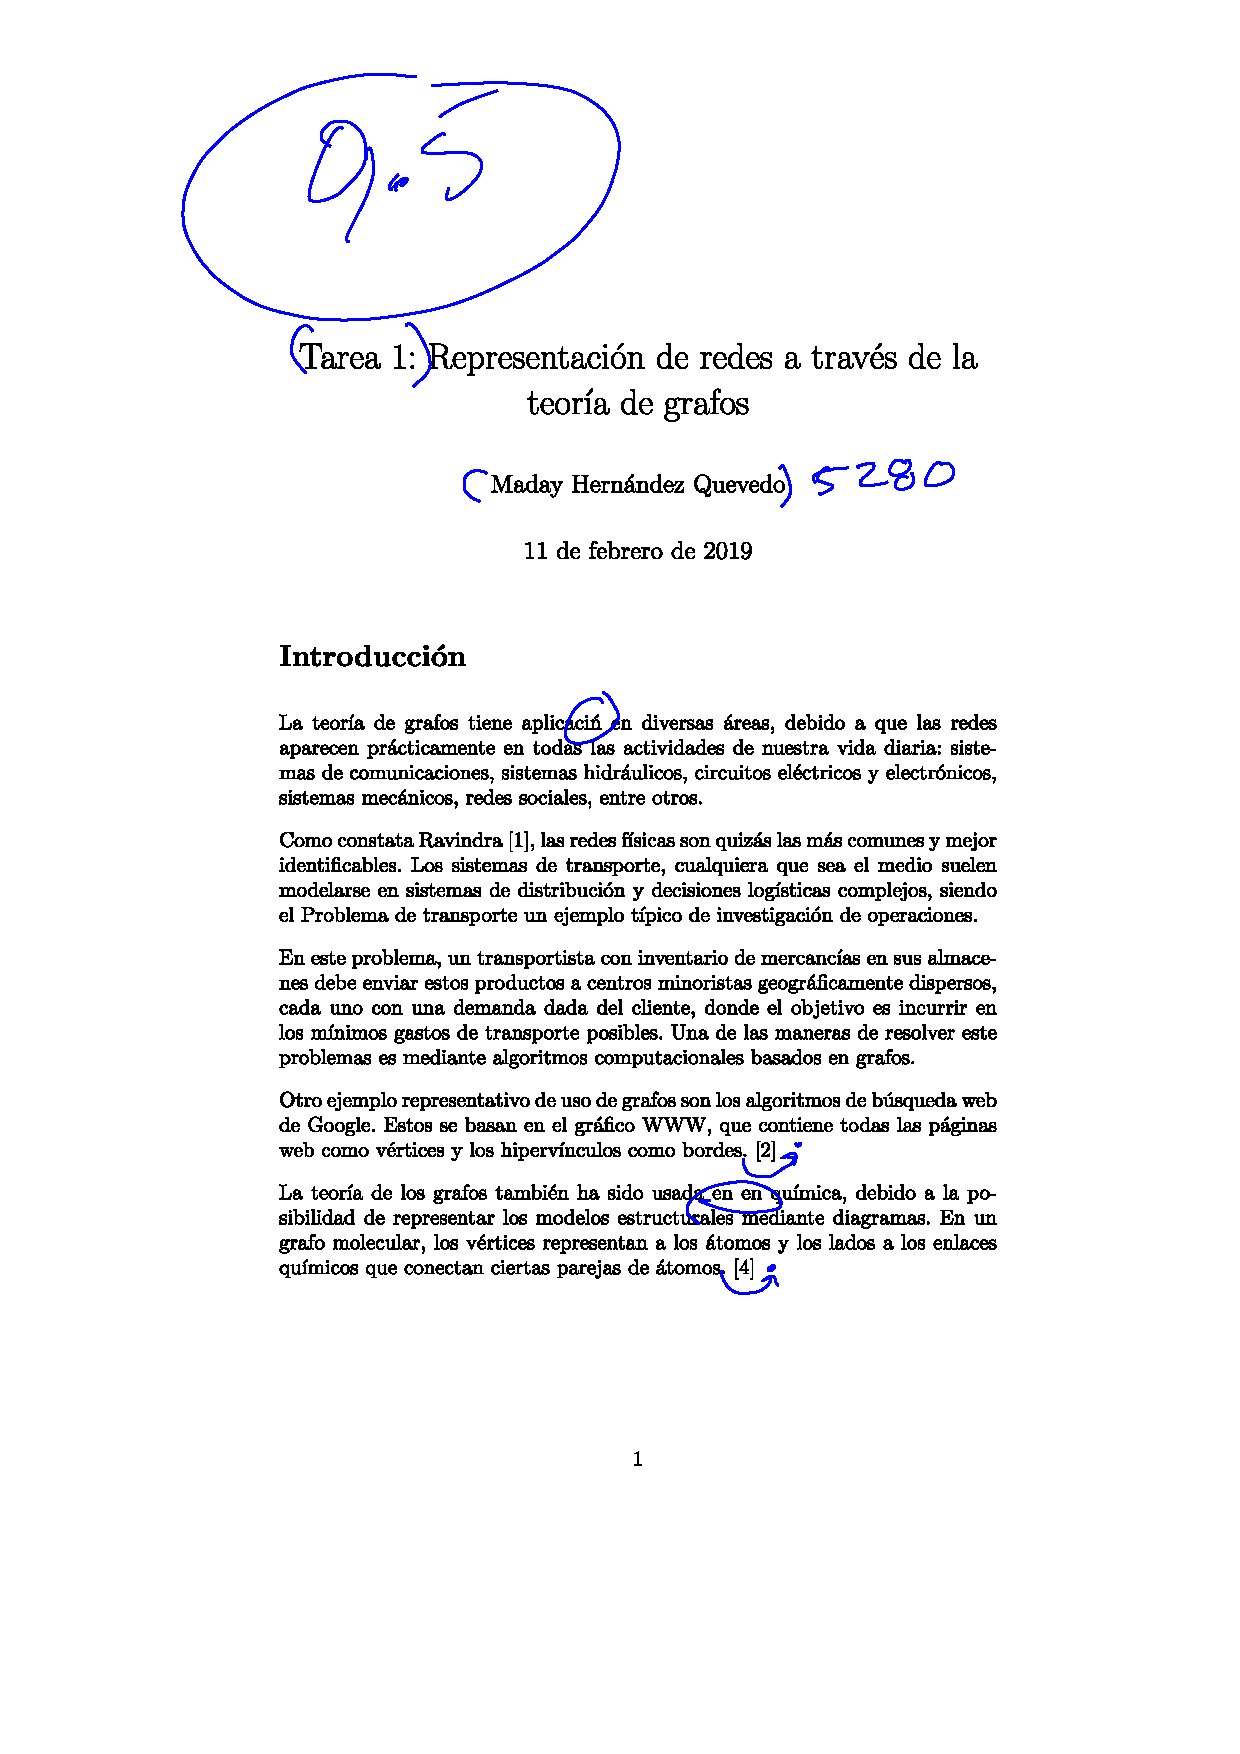
\includepdf[pages=1-22]{pdfrevisados/5280-1.pdf}
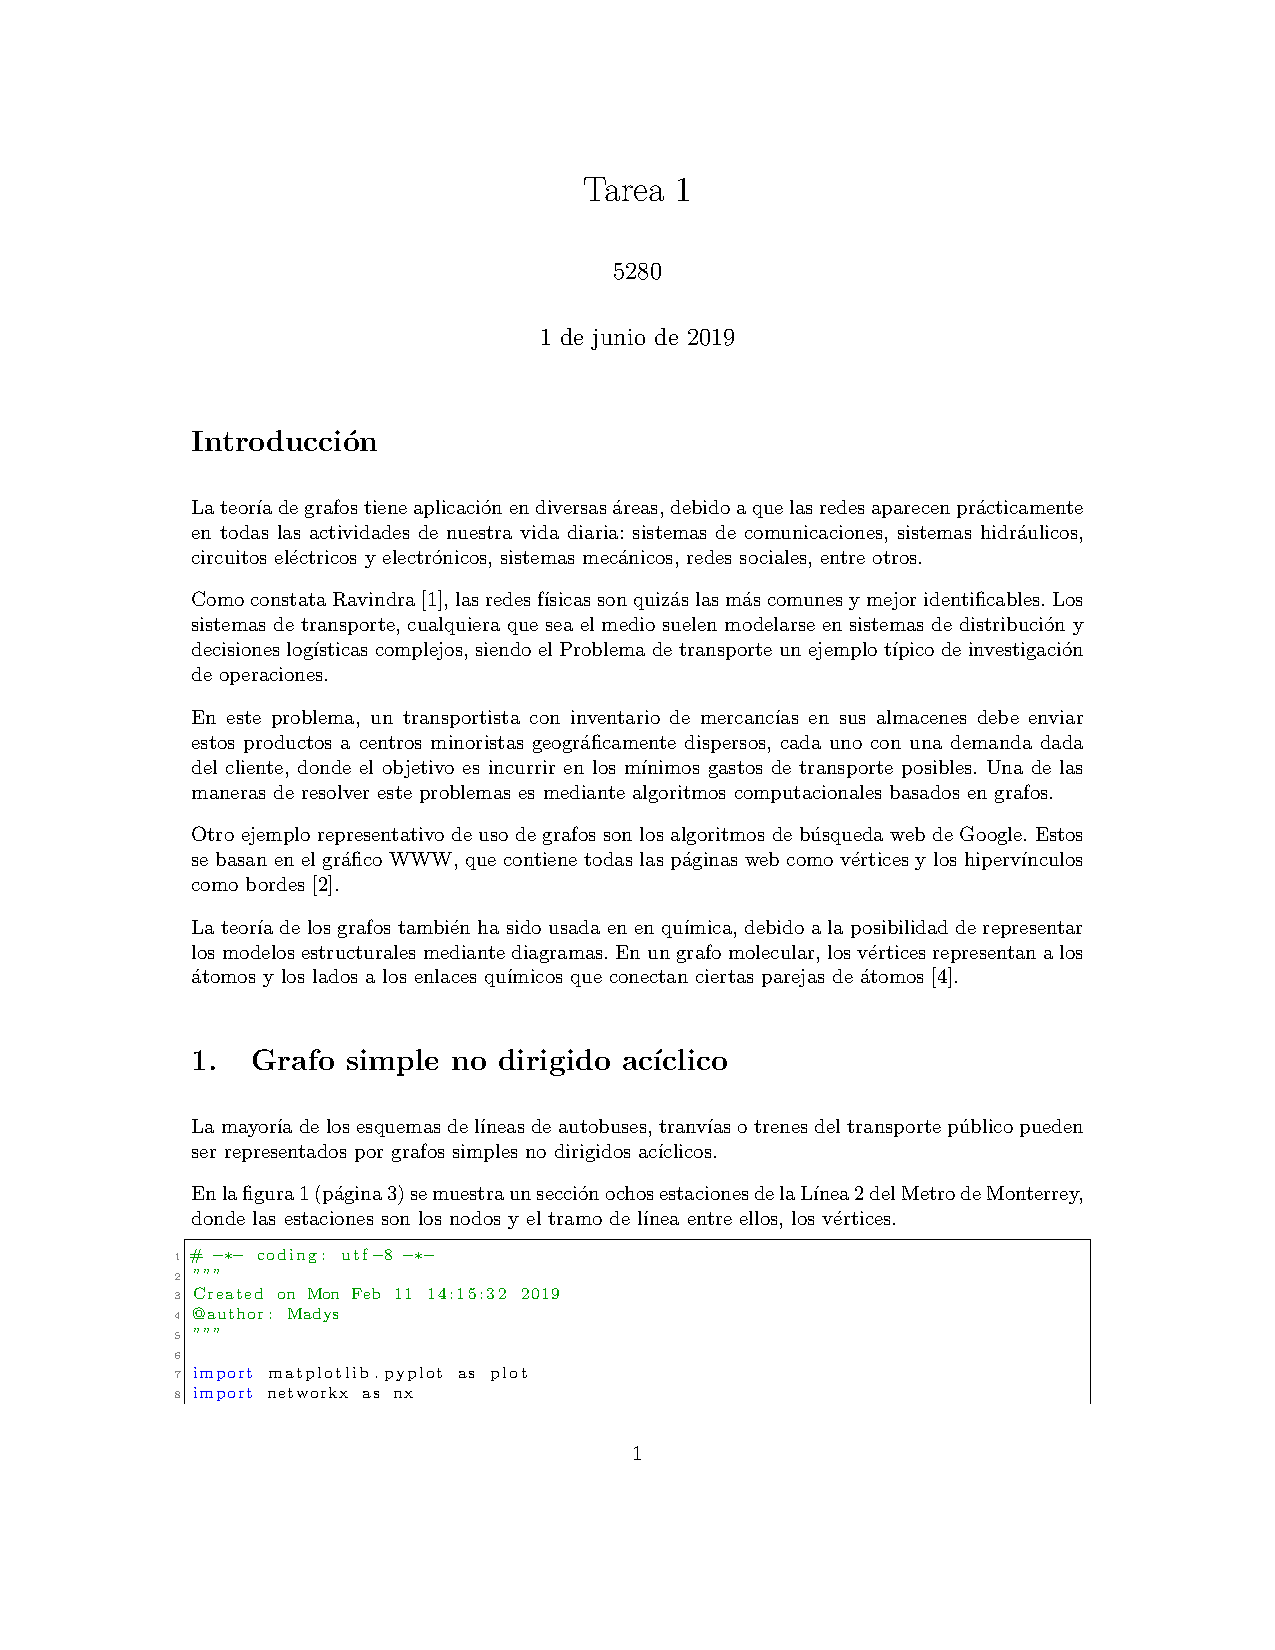
\includepdf[pages=1-18]{pdfrevisados/Tarea1.pdf}
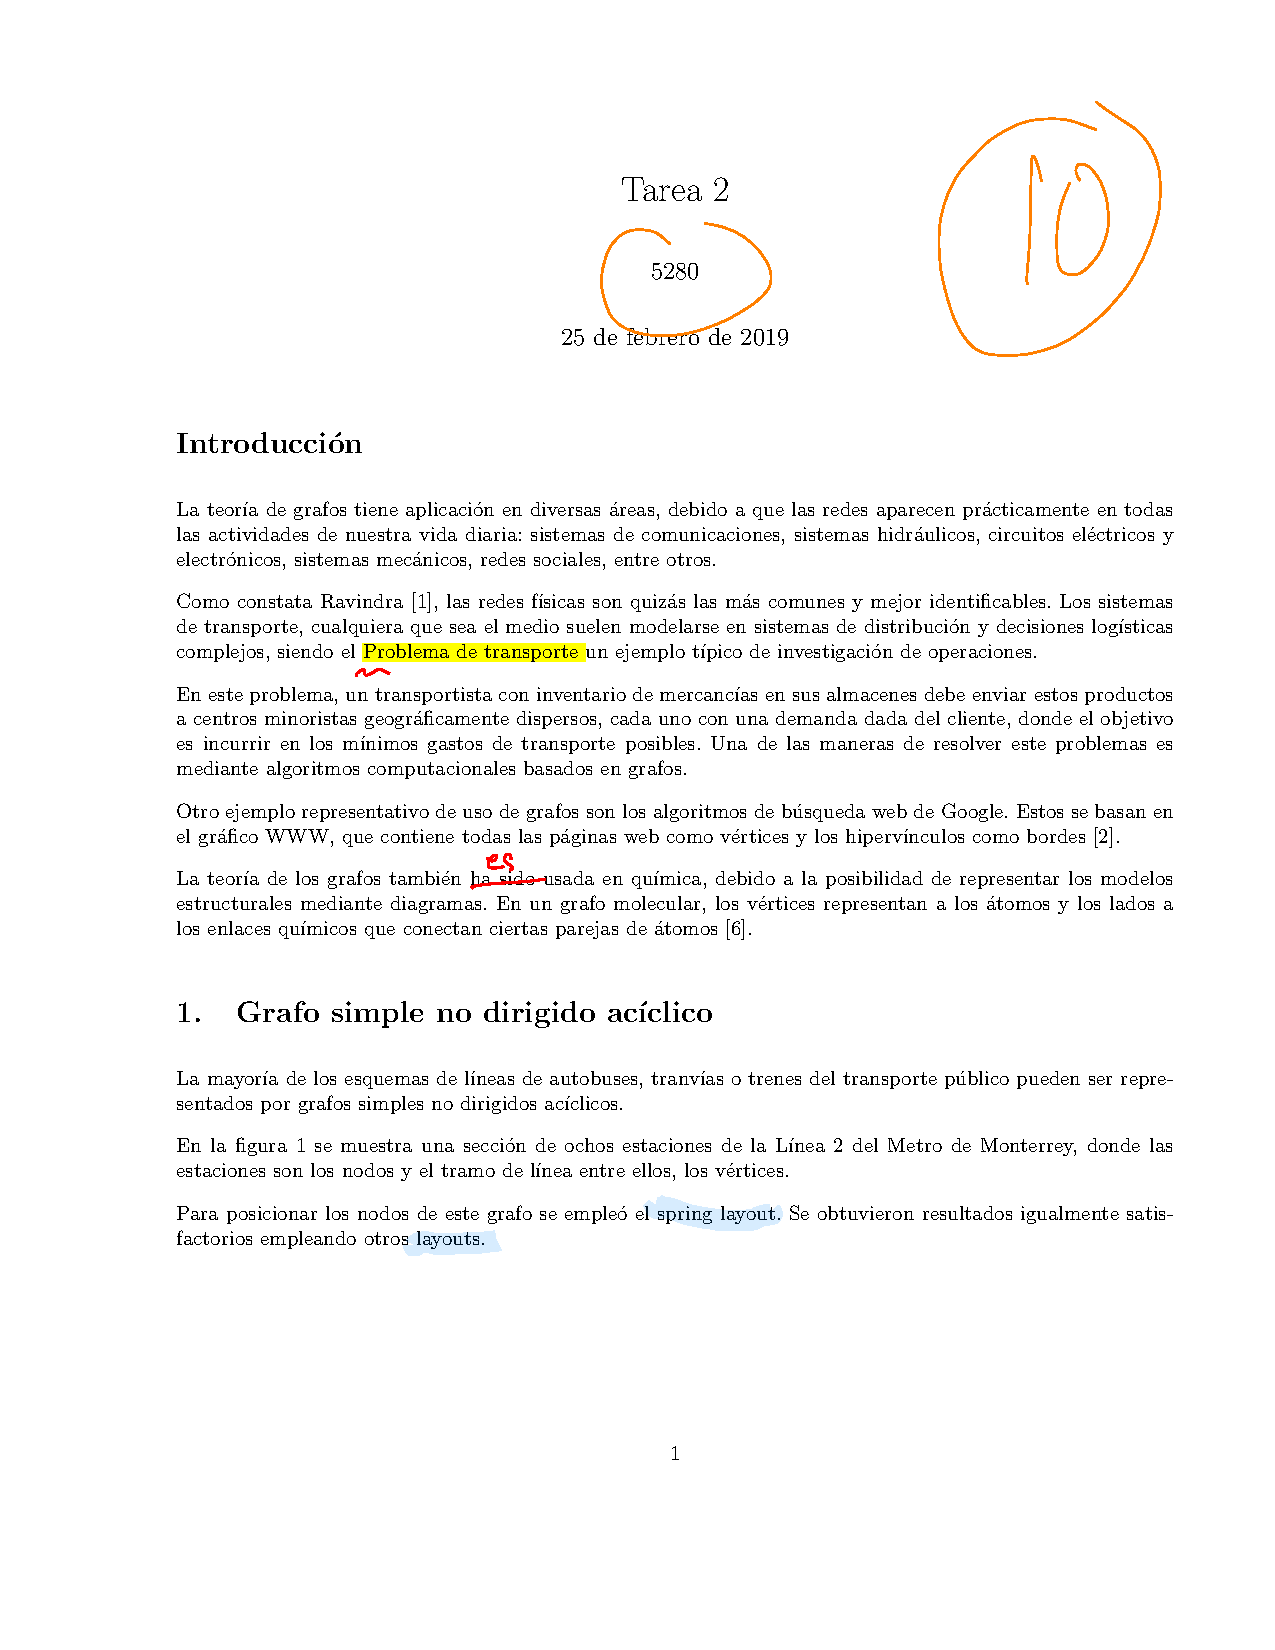
\includepdf[pages=1-18]{pdfrevisados/5280-2.pdf}
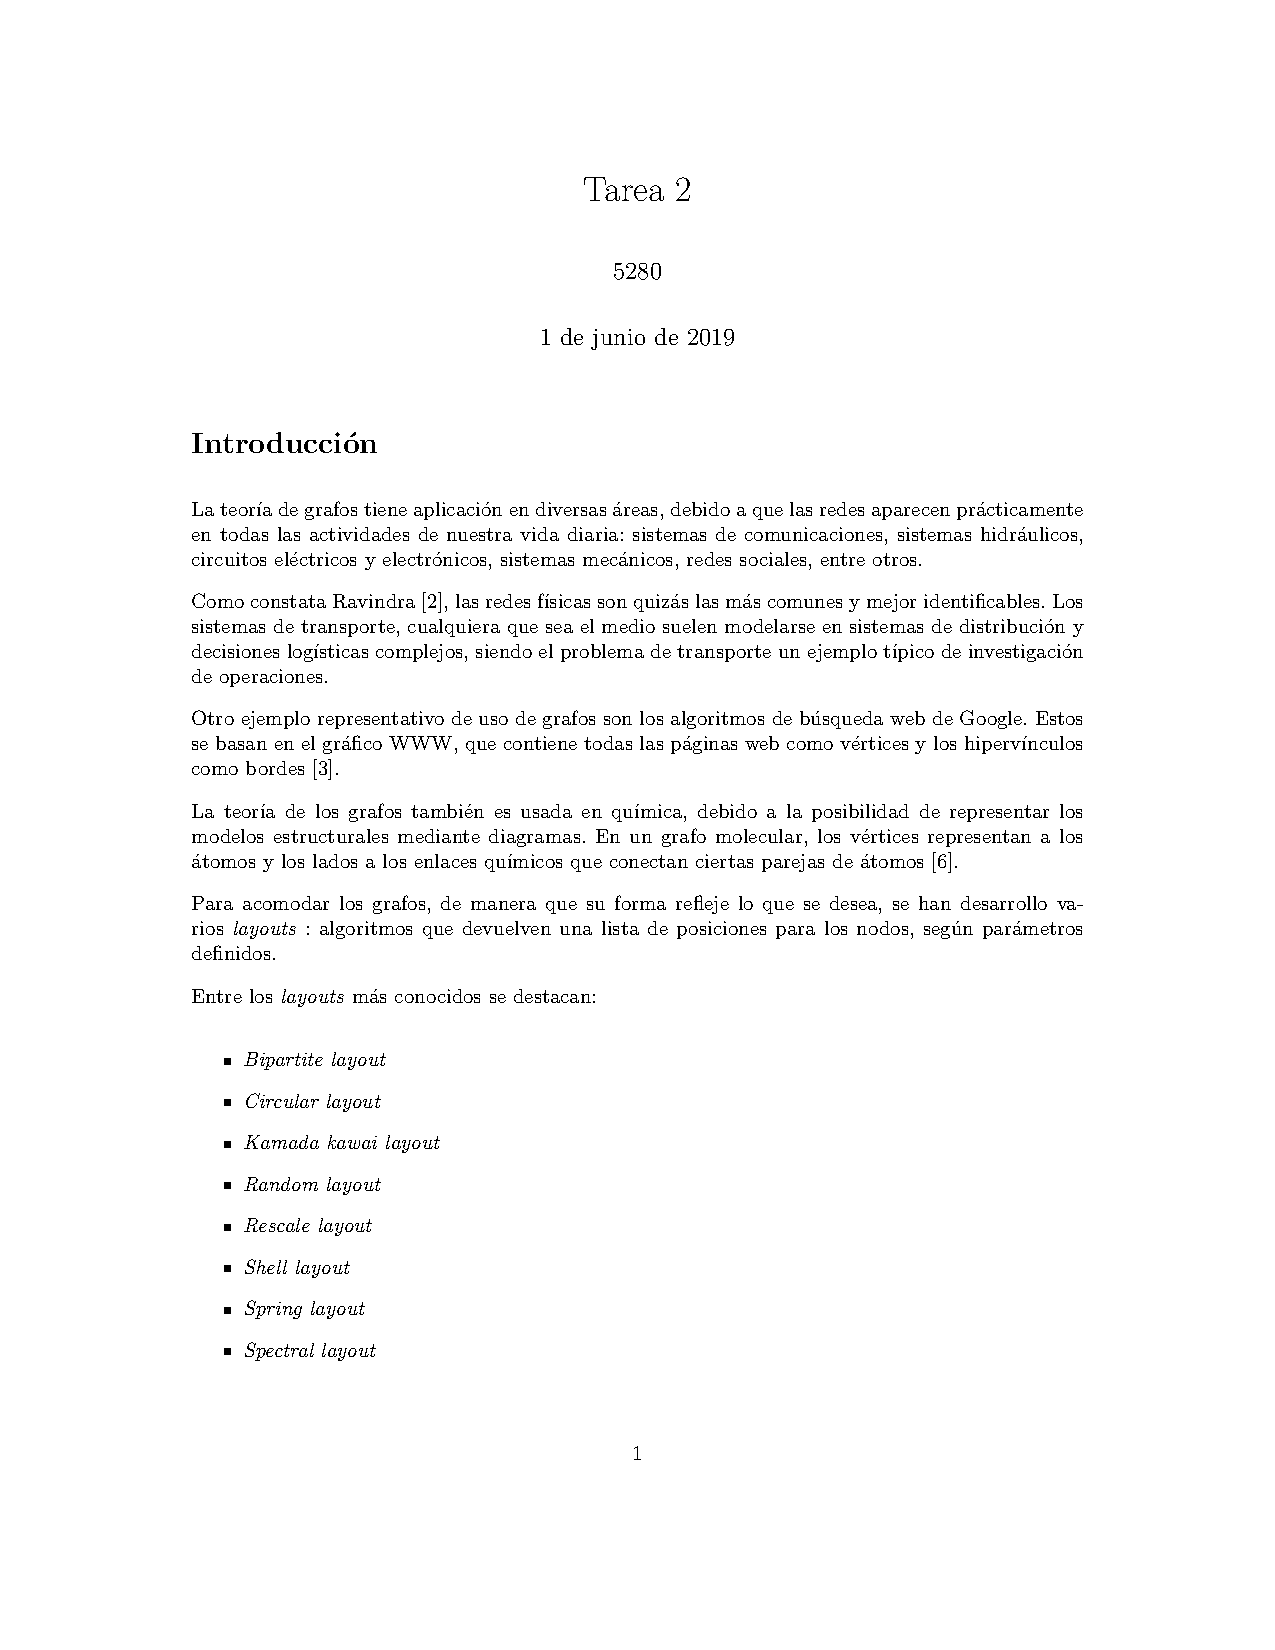
\includepdf[pages=1-17]{pdfrevisados/Tarea2.pdf}
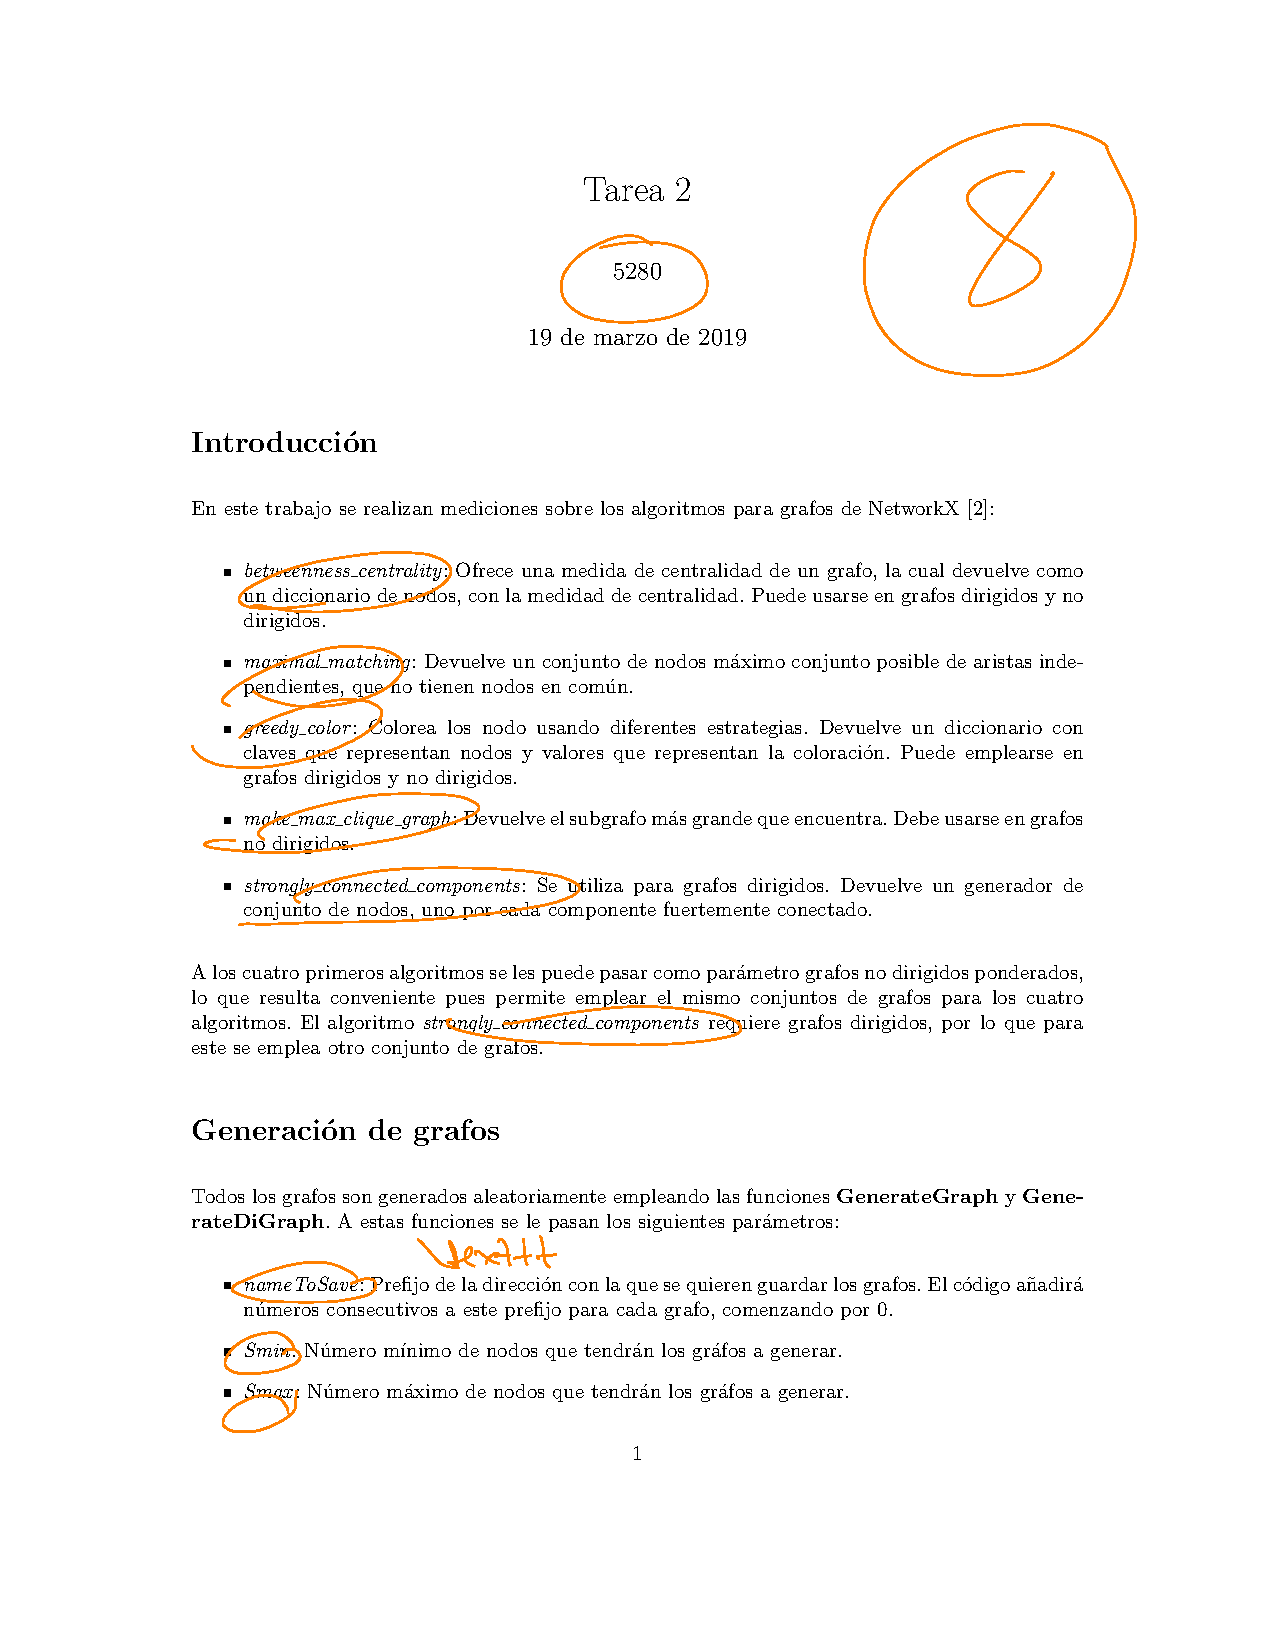
\includepdf[pages=1-7]{pdfrevisados/5280-3.pdf}
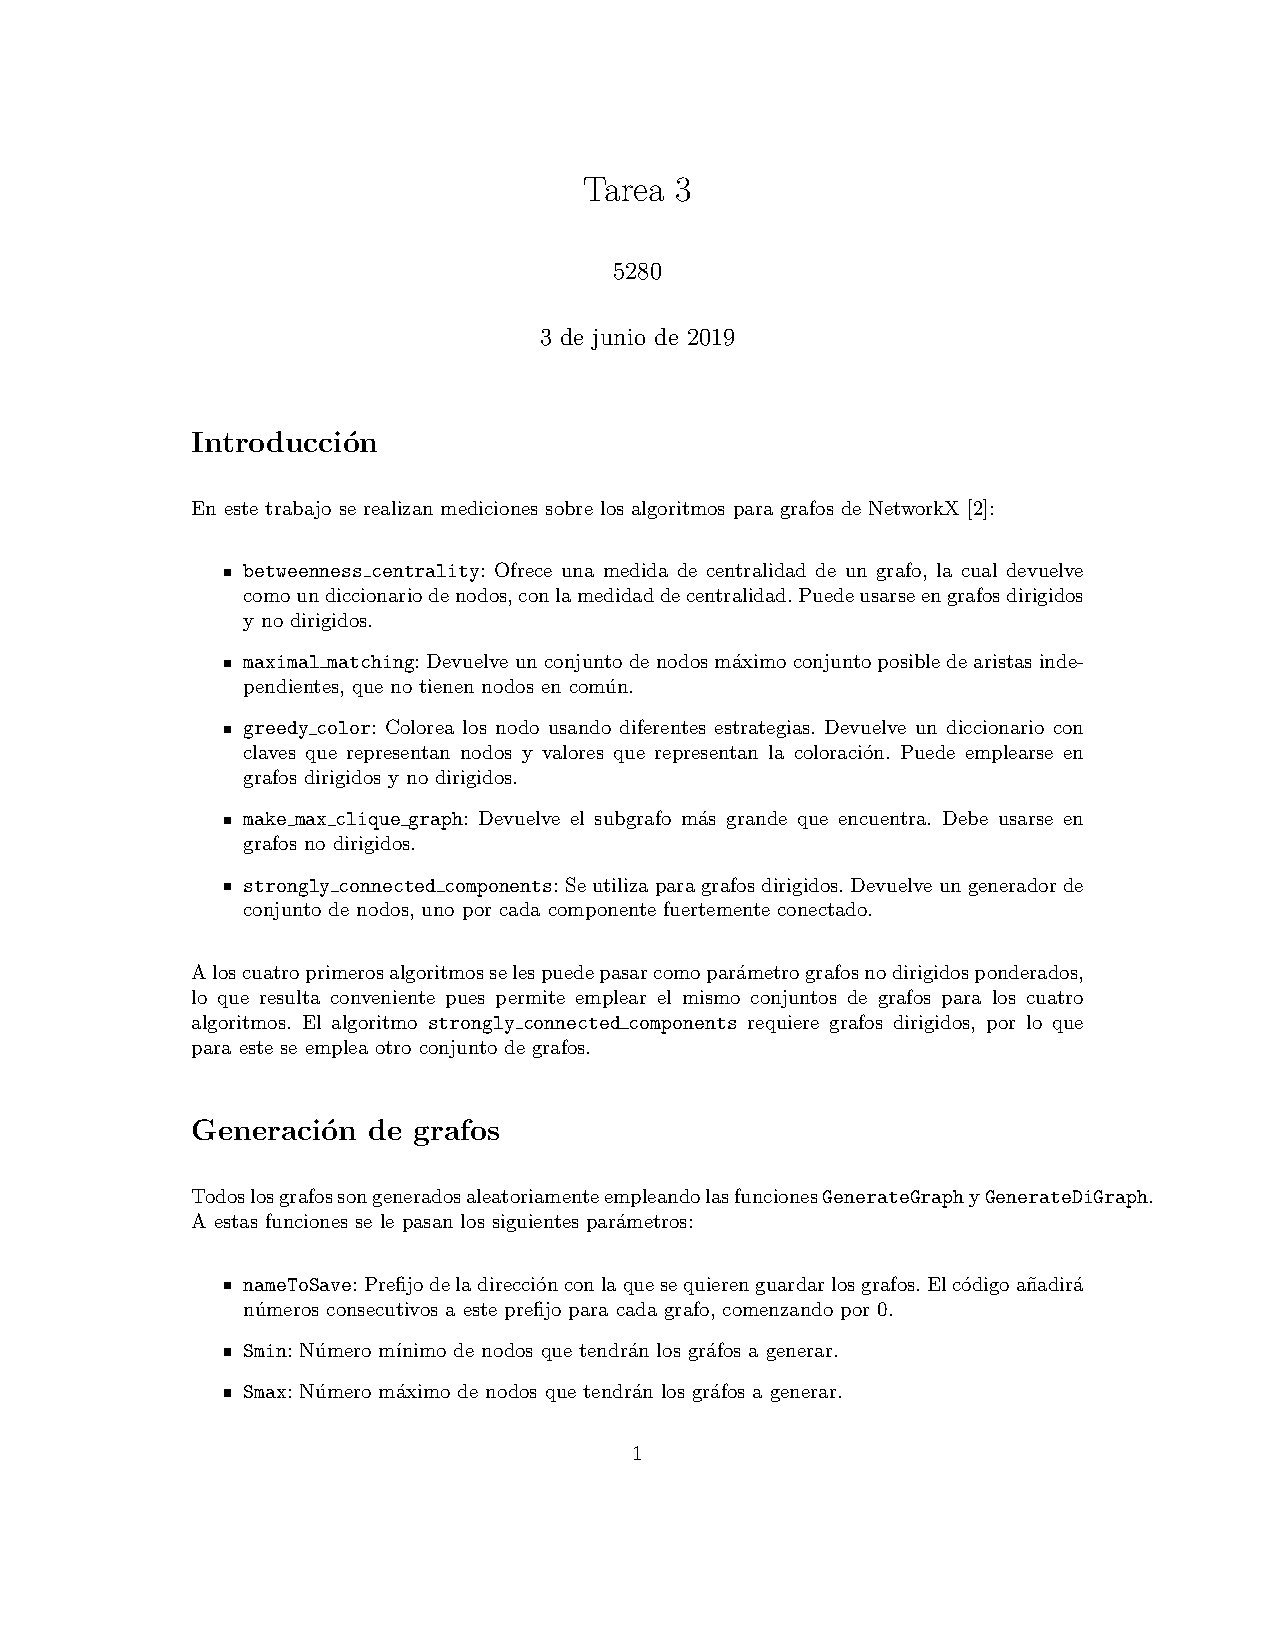
\includepdf[pages=1-8]{pdfrevisados/Tarea3.pdf}
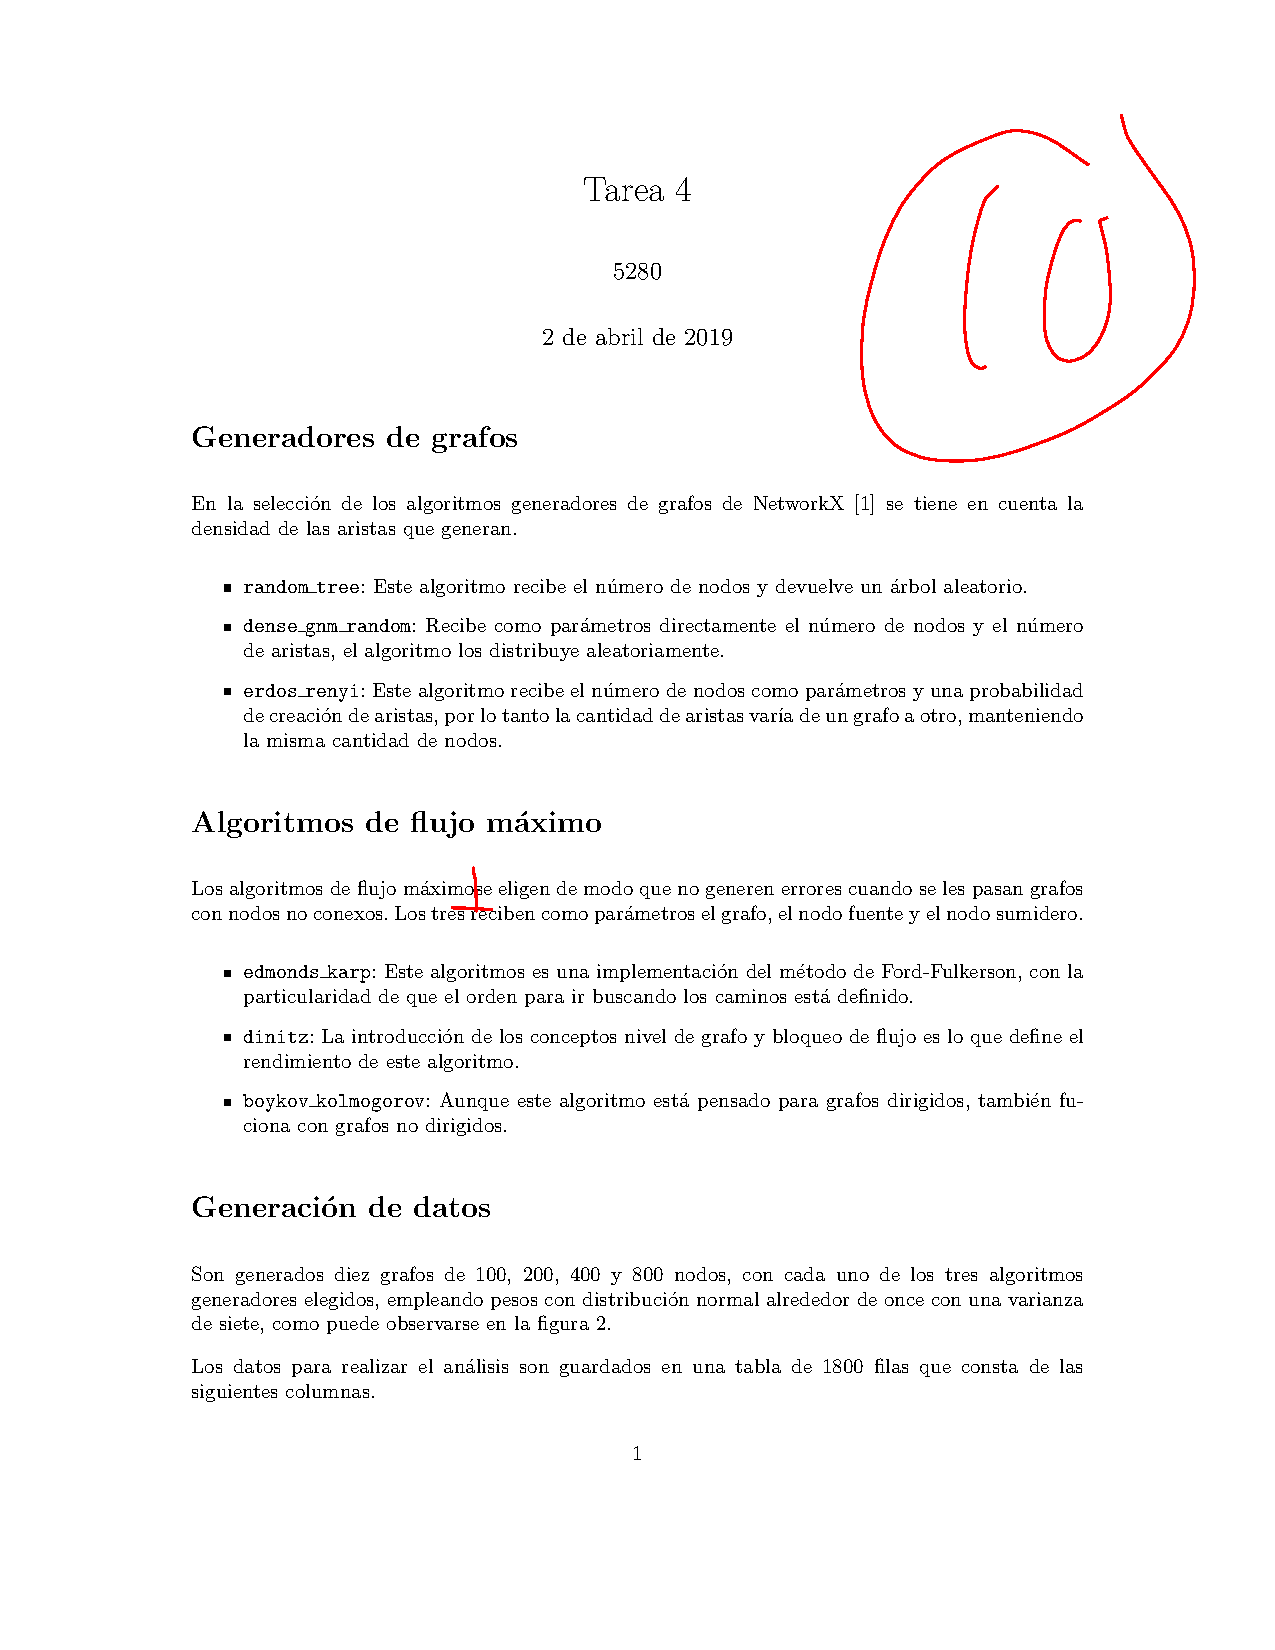
\includepdf[pages=1-9]{pdfrevisados/5280-4.pdf}
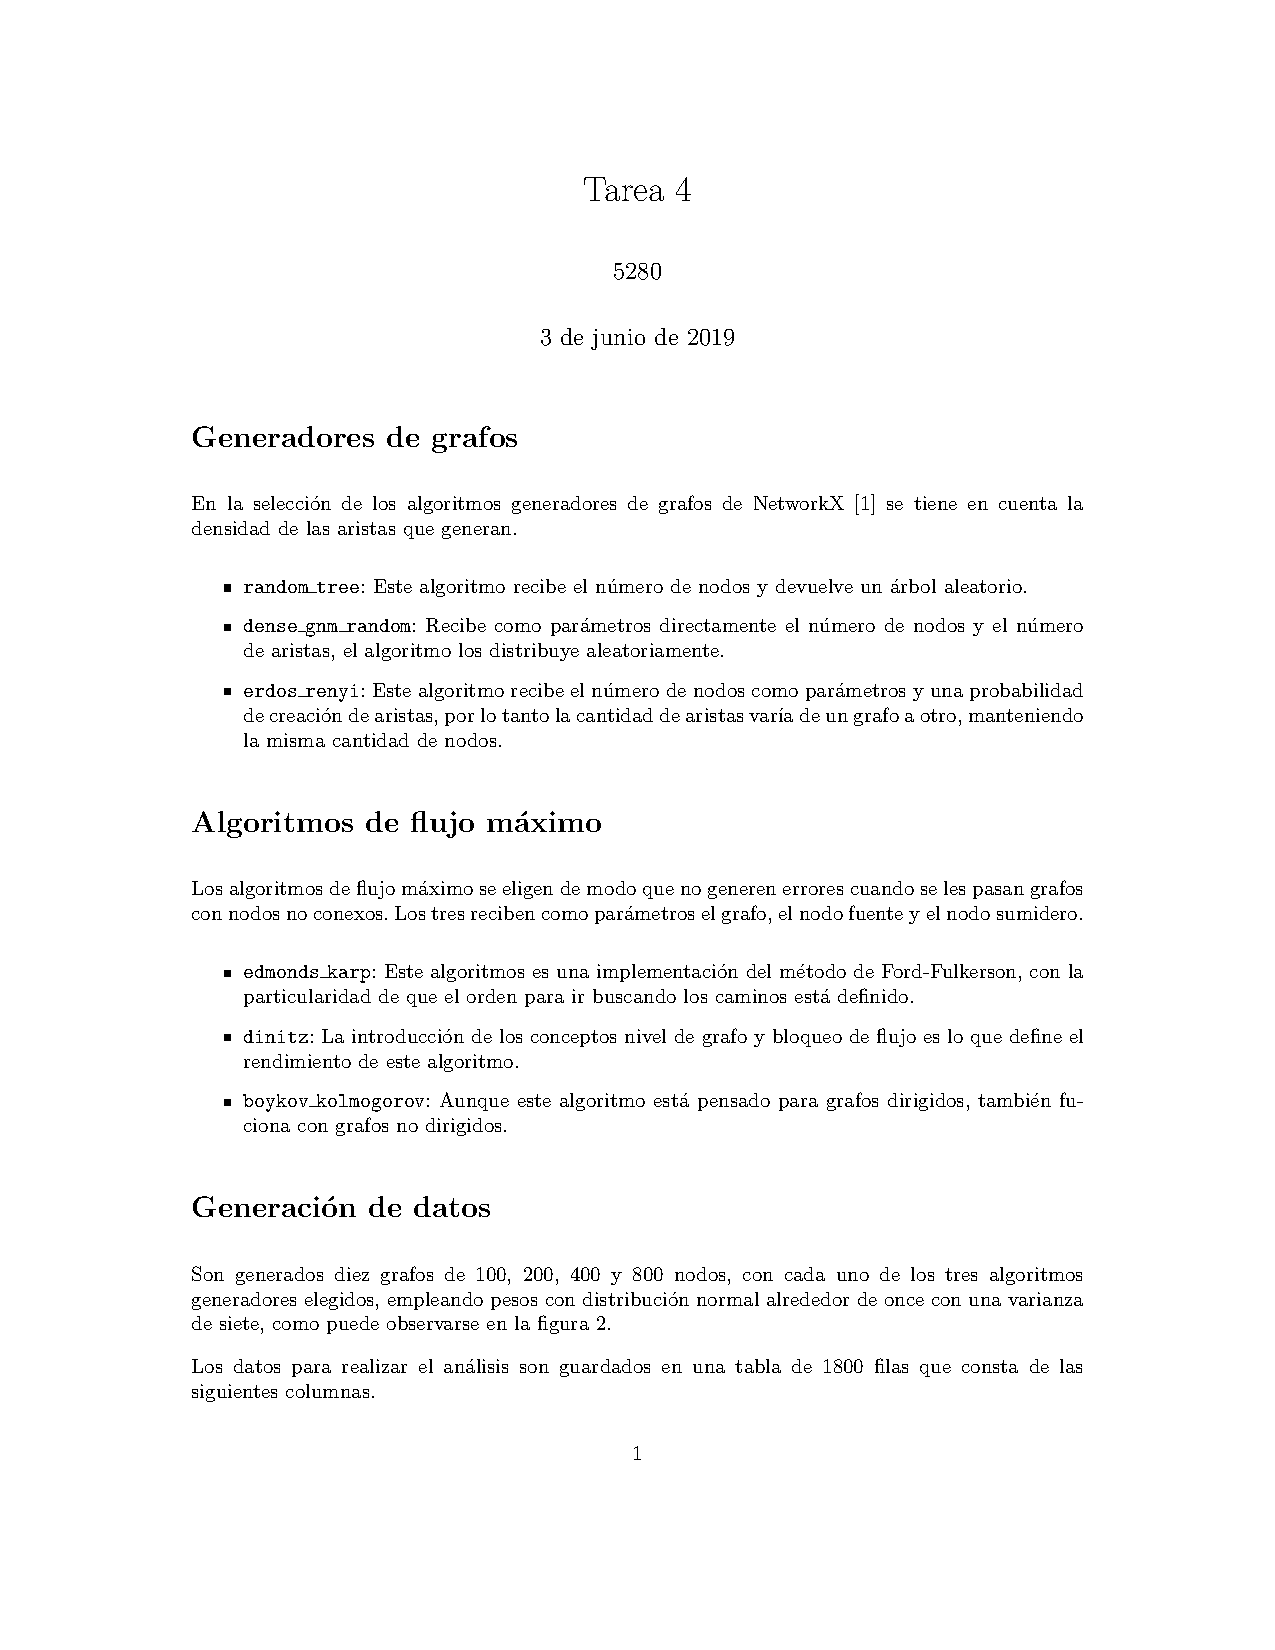
\includepdf[pages=1-9]{pdfrevisados/Tarea4.pdf}
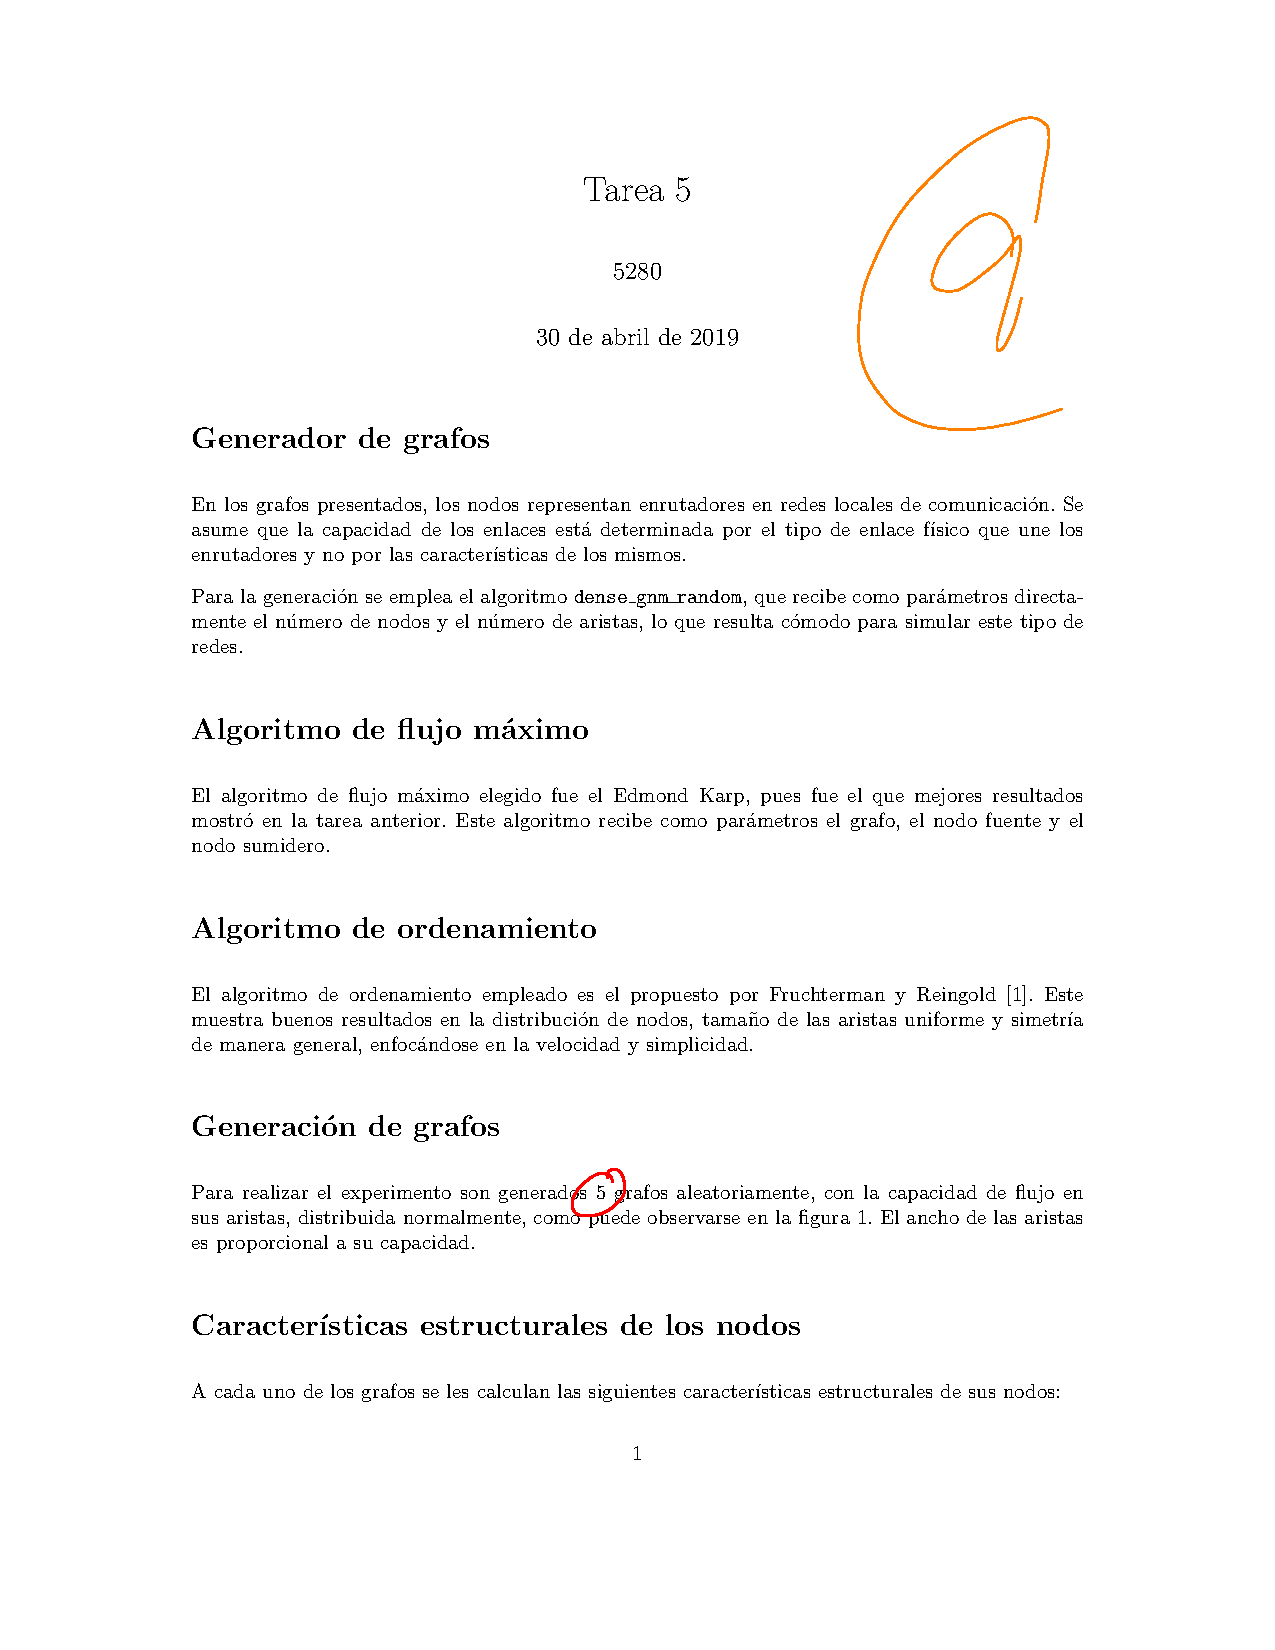
\includepdf[pages=1-12]{pdfrevisados/5280-5.pdf}
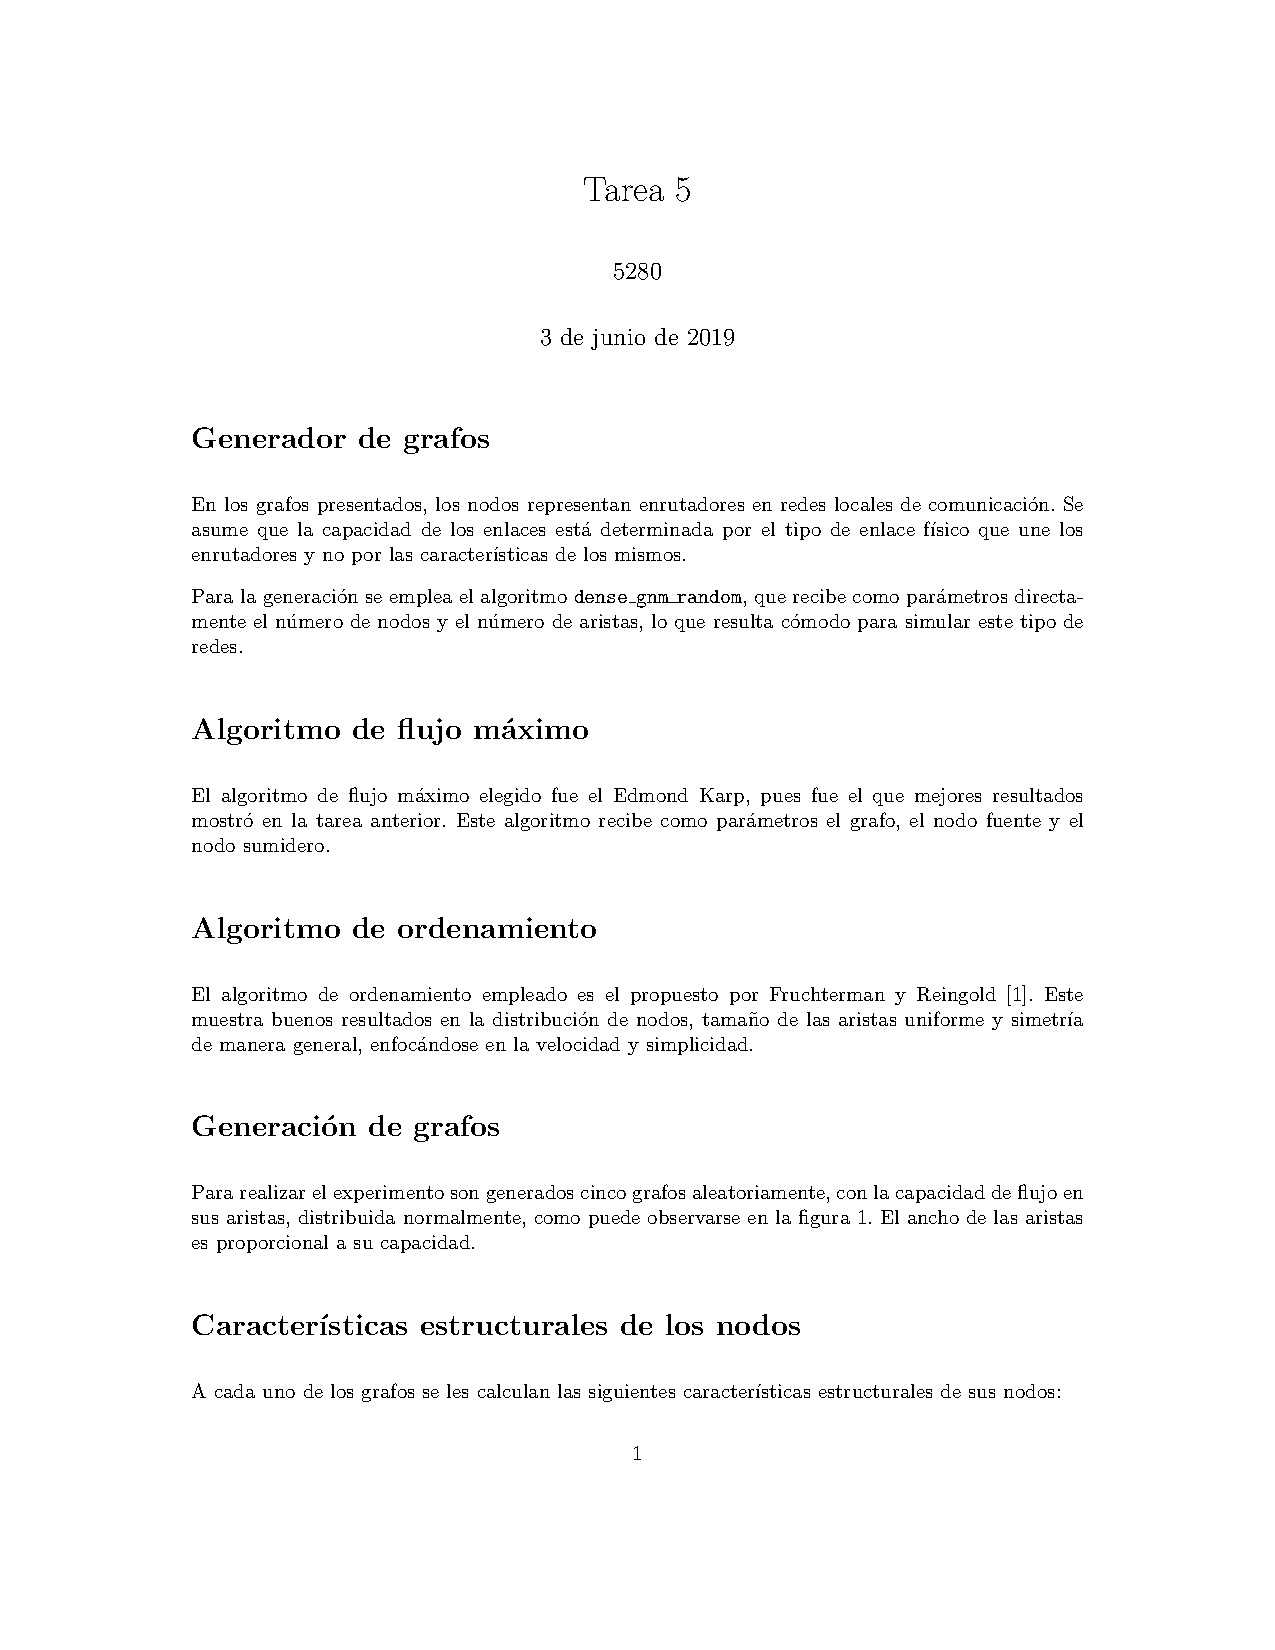
\includepdf[pages=1-12]{pdfrevisados/Tarea5.pdf}

\end{document}